\providecommand{\main}{../../main}
\documentclass[../../main.tex]{subfiles}


\begin{document}

\chapter{Global Trigger Final-OR}
\label{sec:Finor}

\begin{figure}[h]
    \centering
    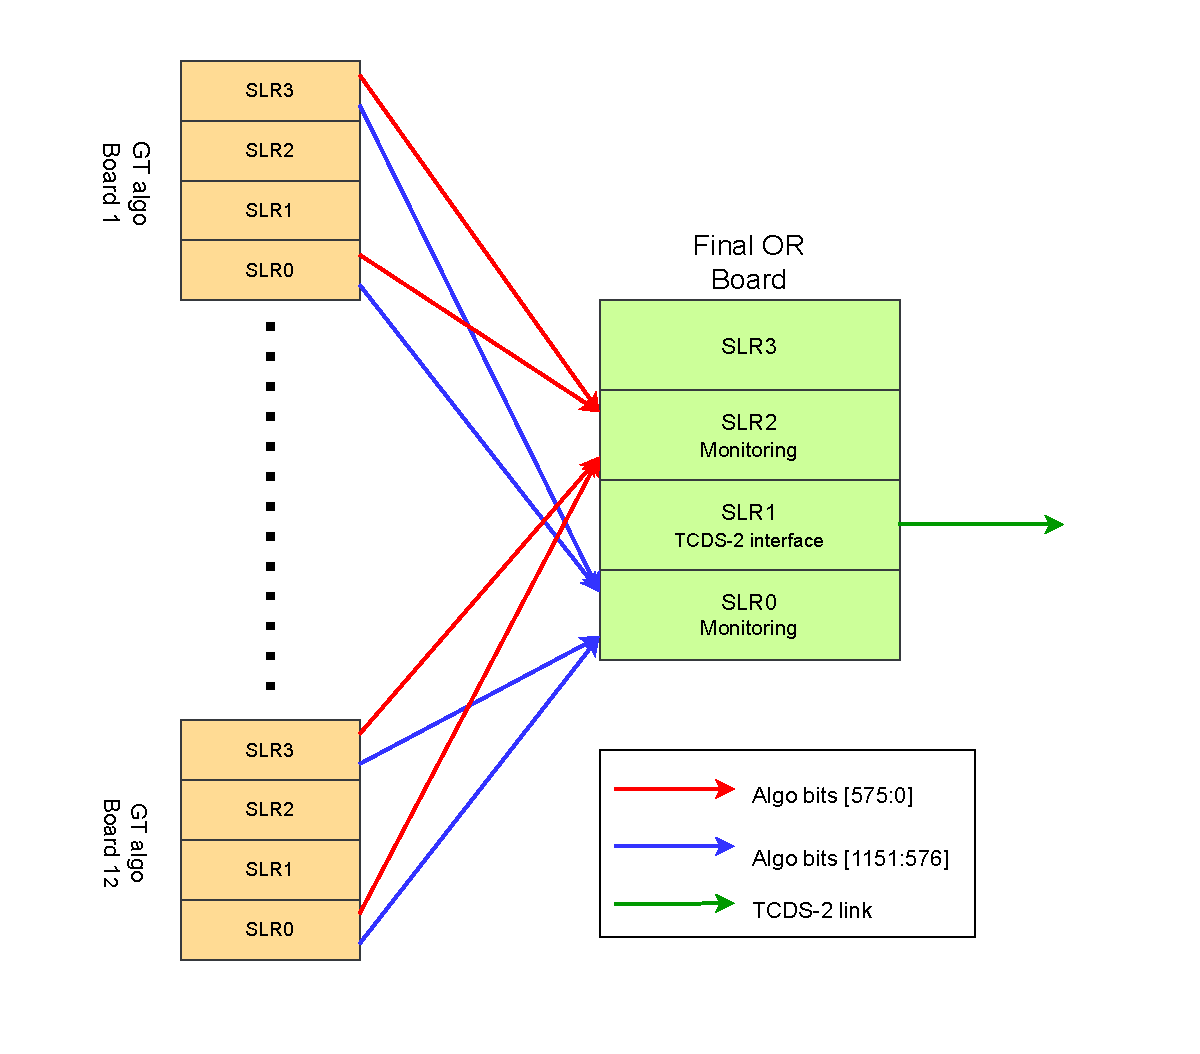
\includegraphics[width=0.85\textwidth]{sections/06/Images/GT_layout.pdf}
    \caption{Global Trigger subsystem structure.}
    \label{fig:GT_layout-finor}
\end{figure}

In this chapter the main features of the Final-OR board (finor-board in the following) are described.  
Each algo-board transmits the bits to the finor-board via 4 links @360MHz, they are arranged in two identical pairs: the first and the third links will carry the lowest 576 bits, the second and the fourth links carry the highest 576 bits. Each algorithm output, during the computation in the algo-board, will be given an index form 0 to 1151 resulting in a wide bus of 1152 bits, one bit for each algorithm output. The Technical Design Report foresees $\sim1000$ algorithms\cite{L1T-2up} and this design is well above such threshold. 

The purpose of such board can be summarized as:
\begin{itemize}
    \item Merge the algo-bits coming from the 12 algo-boards in two 576 wide vectors bit;
    \item Apply masks to the various algorithms following some predefined condition, i.e the bunch crossing mask\footnote{At each bunch number, algorithms are masked for example a mask can be set where there are no collision to avoid potential miss-firing};
    \item Pre-scale each algorithm with a given pre-scale factor (default value is 1).
    \item Extract the algorithms rates;
    \item Produce N different trigger types for different physics programs;
    \item Send the final decision to the Timing and Control Distribution System (TCDS).
\end{itemize}

Before continuing some terms are introduced to better understand how the algorithm monitor logic works. An \textit{orbit} is the proton packets (\textit{bunches}) ensemble that are present in a full LHC revolution. It is made up of 3564 \textit{bunches} and each bunch is 25ns apart, by extent the main frequency is 40MHz usually referred as \textit{LHC clock}. The counters within the Finor-board take as reference the LHC clock: 
\begin{itemize}
    \item the bunch counter will be increased at each LHC clock rising edge;
    \item the orbit counter will increase when the bunch counter reaches the value 3564;
    \item the \textit{luminosity section} last a given number of orbits, in this case this number is set to $2^{19}$ orbits\footnote{that corresponds to $\sim 46.6s$}, from this definition the begin luminosity section definition follows, this signal is asserted for exactly one LHC clock cycle at the beginning of each luminosity section.
\end{itemize}

\section{Final-OR board structure}
\label{sec:Finor_struct}

\begin{wrapfigure}{r}{0.45\textwidth}
    \centering
    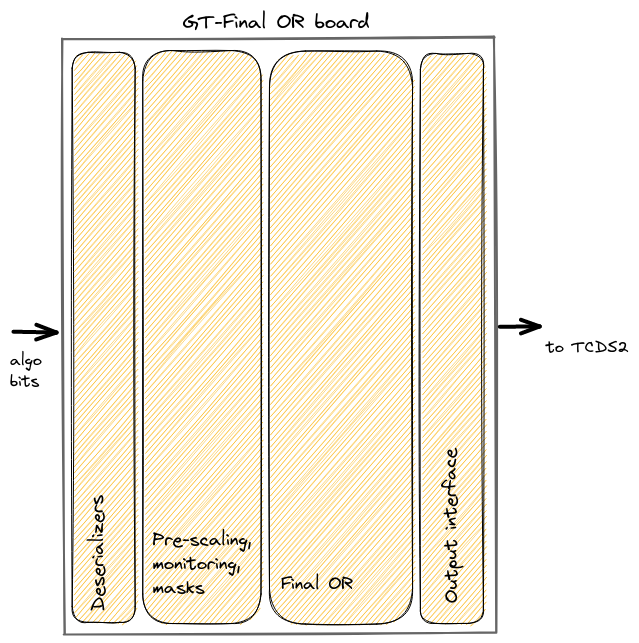
\includegraphics[width=0.45\textwidth]{sections/06/Images/GT-finor.png}
    \caption{GT-Final OR board structure.}
    \label{fig:GT-finor}
    %\vspace{1cm}
\end{wrapfigure}

The requirements for the VHDL code that has to be developed are explained in this section. 
Modules need to be split in to two different blocks due to resource limitation in a single SLR, this is done to reduce to a minimum potential timing violations.  

The finor-board design sketched in Fig. \ref{fig:GT-finor} and \ref{fig:Finor_struct}  will be split in SLR substructures to minimize potential timings violation due to the communications between different SLRs:
\begin{itemize}
    \item \textbf{SLR$_0$}: In this SLR the 24 input links are merged together to get the highest 576 bits ([1151:576]), then the monitor logic and pre-scale logic act on such wide bit vector and finally the local trigger bits are computed.
    \item \textbf{SLR$_1$}: SLR devoted to the final OR of the trigger decisions coming from the two monitoring SLRs. The TCDS-2 interface will be placed here, right after the local OR. 
    \item \textbf{SLR$_2$}: Same structure of the SLR$_0$, but in this case the lowest 576 bits ([575:0]) are the target.
    \item \textbf{SLR$_3$}: This SLR is left empty for future features implementations. 
\end{itemize}

\begin{figure}[h]
    \centering
    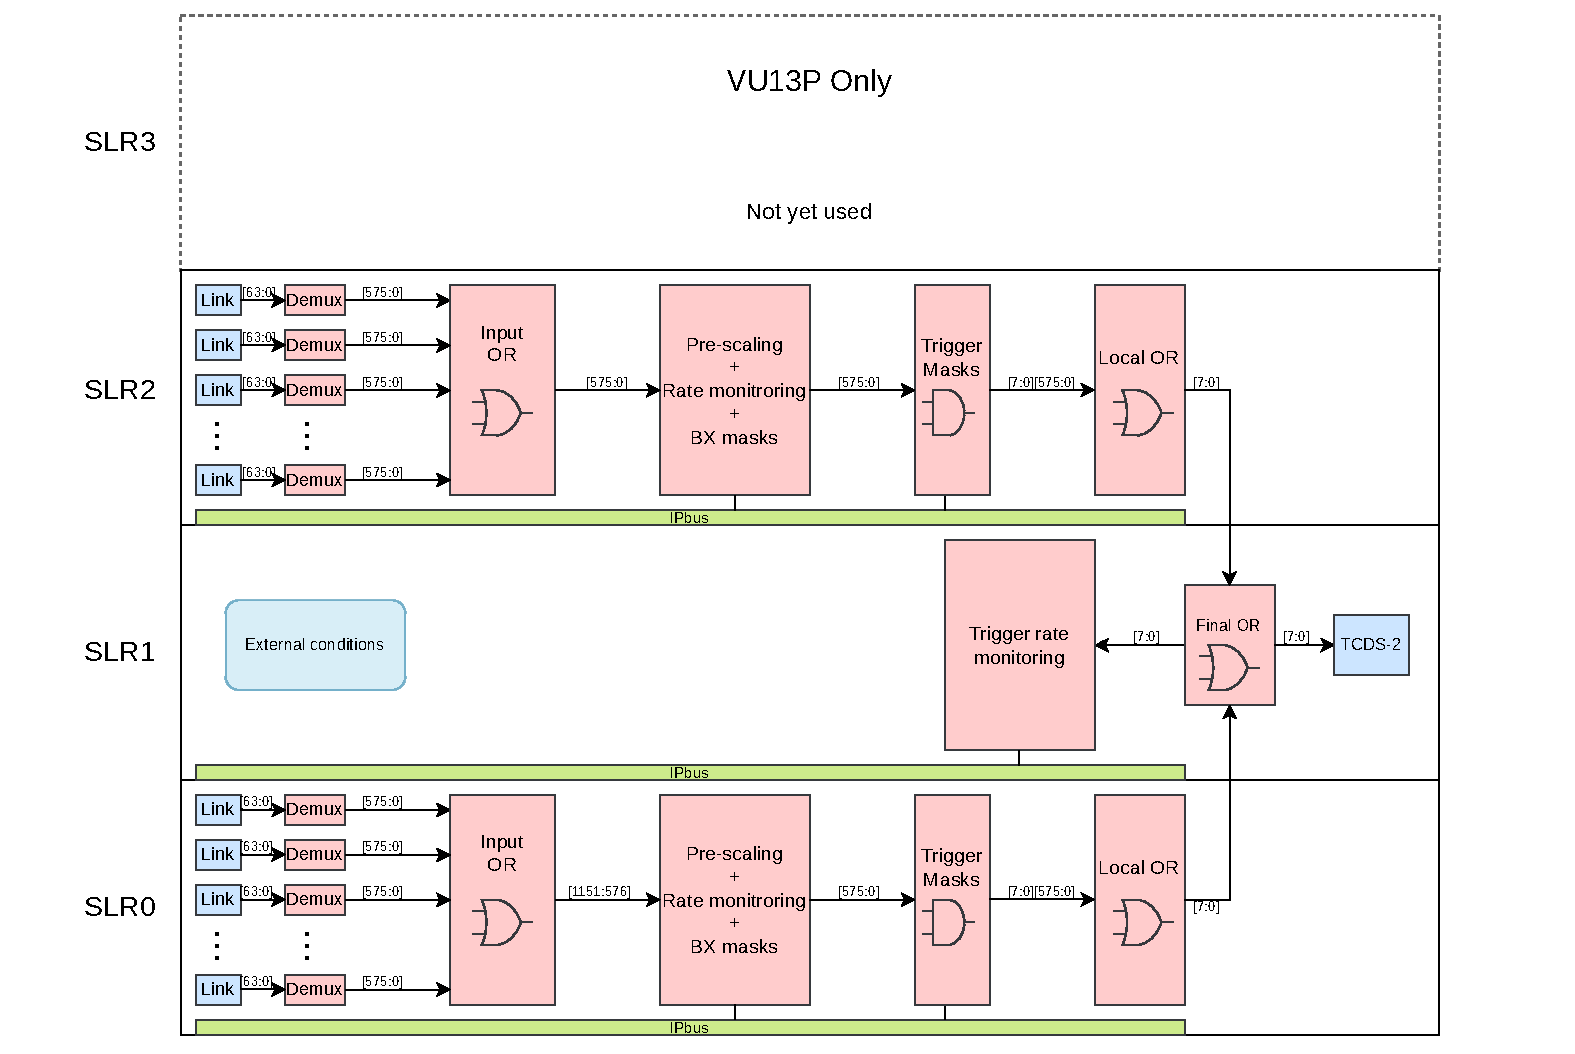
\includegraphics[width=0.9\textwidth]{sections/06/Images/SLRS_layout.pdf}
    \caption{Final-OR design layout, each SLR architecture is kept isolated as much as possible from the others to reach timing closure, the only signal that cross SLRs is the trigger decision bit array.}
    \label{fig:Finor_struct}
\end{figure}

Each algorithm monitor logic is encapsulated in a module called \textit{algo\_slice}, its structure is shown in Fig \ref{fig:Algo_slice}, it counts two pre-scalers, three rate counters and one post-dead time rate counter. The figure highlights one of the many optimizations introduced on the existing logic. In this particular example the L1A signal delay logic has been merged together, in this way instead of using a high number of shift registers only a BRAM is used, reducing both the resource usage and route congestion.

\begin{figure}[h]
    \centering
    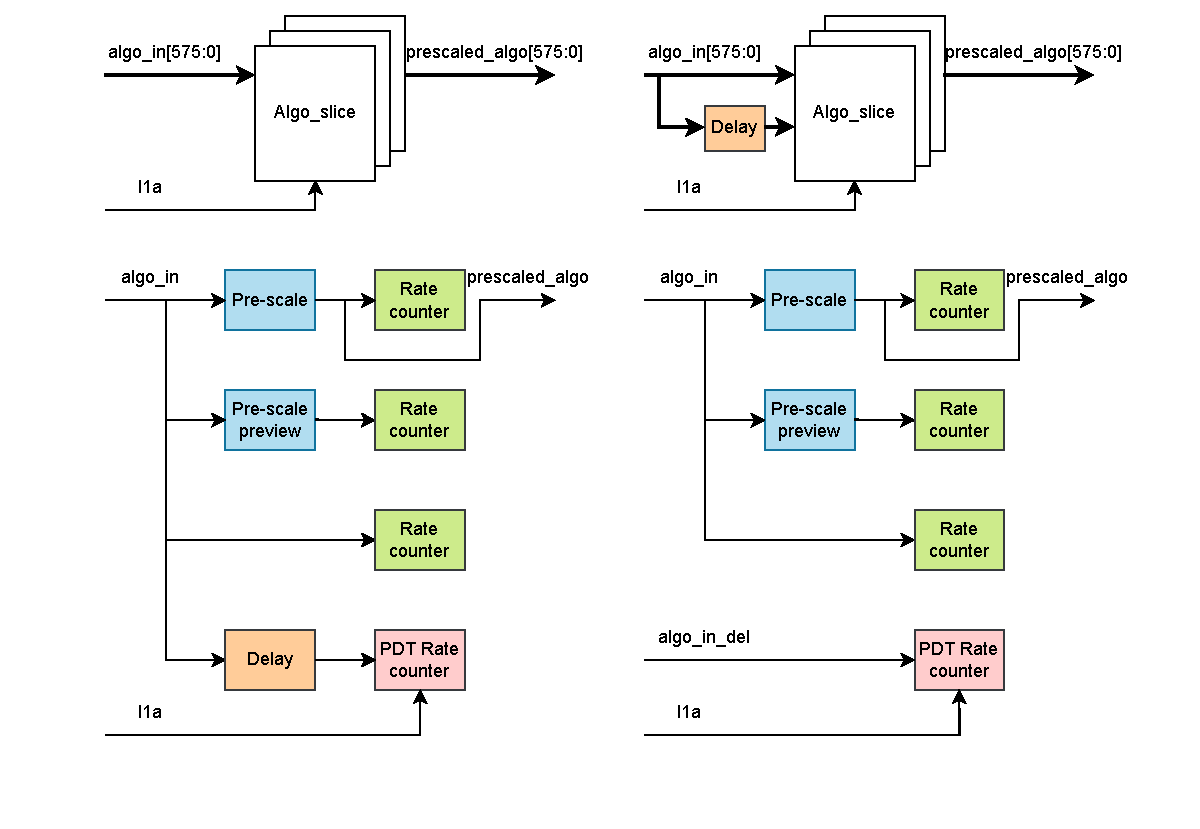
\includegraphics[width=0.95\textwidth]{sections/06/Images/Algo_slice_mod.pdf}
    \caption{Algo\_slice architecture, particular optimization on the delay line}
    \label{fig:Algo_slice}
\end{figure}

In the following the main modules are explained in detail.

\subsection{IPbus protocol}
\label{sec:IPbus}

\begin{figure}[h]
    \centering
    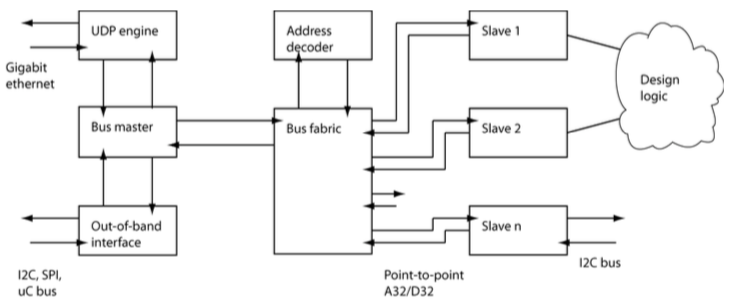
\includegraphics[width=0.57\textwidth]{sections/06/Images/bus_topology.png}
    \caption{Bus topology of the IPbus suite, multiple choice to interface with the host machine are available: ethernet, PCIe or Axi-lite. The communication with the design can be made with RAM, ROM or registers.   }
    \label{fig:Ipbus}
\end{figure}

A key firmware element is the IPbus protocol\cite{IPbus}, this tool was developed with the objective of a reliable high-performance control link for particle physics electronics. The IPbus protocol is a simple packet-based control protocol for reading and modifying memory-mapped resources within FPGA-based hardware devices which have a virtual A32/D32\footnote{32-bits wide address bus and 32-bits wide data bus} bus.   

The memory-mapped resources can be RAM, ROM or simple registers; in the finor-board multiple modules with an IPbus connection are used:
\begin{itemize}
    \item RAM to store the pre-scale factors, software write and hardware read;
    \item RAM to store the trigger masks and bunch crossing masks, software write and hardware read;
    \item RAM to store the rate counter value, hardware write and software read;
    \item General purpose registers to read and write status and control flags.
\end{itemize}

\subsection{Algorithm pre-scaling}
\label{sec:Finor_presc}

The pre-scale module developed by the Global Trigger group for the $\mu$GT has been modified, but the main logic stayed the same \cite{uGT}. The new module has been heavily optimized to reduce the resource foot print in order to reach the goal of 1152 total algorithms. Such optimization range from simple logic rearrangement to signal vectorization. The loading of the pre-scaler values is pictured in Fig. \ref{fig:Pre-scaler-load} where it is used a dual port ram to store the values, at each luminosity section the RAM is read and the values are stored in a register array, in the next luminosity section if the request update flag is asserted the factors are loaded inside the algo-slices.

\begin{figure}[h]
    \centering
    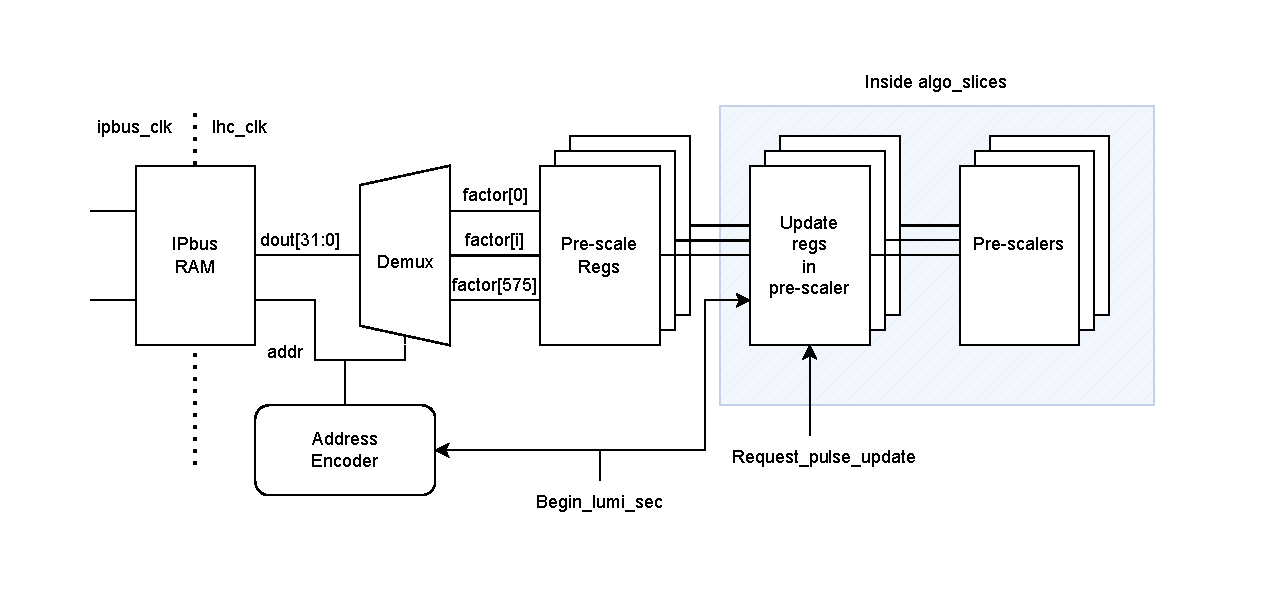
\includegraphics[width=0.8\textwidth]{sections/06/Images/Presc_fact_reg.pdf}
    \caption{Optimization in the pre-scale factors loading.}
    \label{fig:Pre-scaler-load}
\end{figure}

Every algorithm has a pre-scaler with a pre-scale factor 24 bits wide\footnote{This number can be increased up to 32 bits}. This module reduces the trigger-rate of the incoming algorithm by a given factor that can be set via software. For example a factor of 3 lets every third trigger pass blocking the first two.\newline 
A new feature introduced in 2019 is the possibility to set a fractional factor, each factor will be defined with an integer part and two digit fractional values. An example waveform with a factor of $1.75$ is shown in Fig. \ref{fig:prescaler}.\newline
The counter's increment of each algorithm assertion is $100$, in fact with two fractional digit this corresponds to exactly $1$. The factor of this example is $1.75$, if the counter plus the increment is greater or equal to the pre-scale factor the algo\_prescale flag is asserted and the counter is decreased by the pre-scale factor value.


\begin{figure}[h]
    \centering
    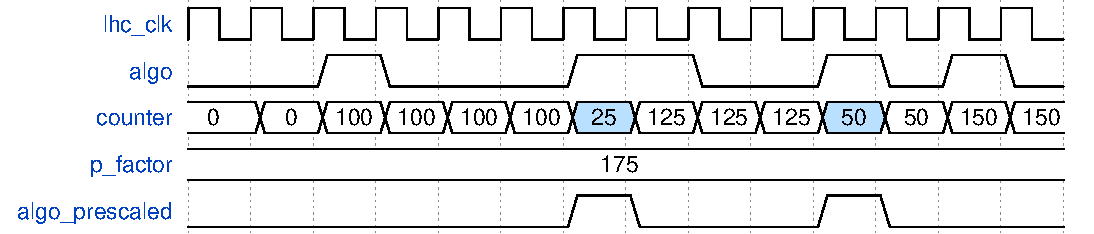
\includegraphics[width=0.93\textwidth]{sections/06/Images/Prescaler_wf_1.pdf}
    \caption{Pre-scaler counter increment waveform.}
    \label{fig:prescaler}
\end{figure}

Each algorithm has two pre-scaler, the first is the effective pre-scale, the second is used as a preview to evaluate the result with a second pre-scale factor.

\subsection{Algorithm rate counters}
\label{sec:Finor_ratecnt}

The rate counters are used to extract the rate of each algorithm for monitoring purposes, in fact as was described in section \ref{sec:L1T}, the level-1 trigger has a maximum accept rate and it is useful to have a monitor to spot potential rate mismatch with the expected values. 

The counter is increased at each LHC clock cycle if the input algorithm is asserted while the reset condition is the start of a luminosity section or an external signal. Right before the reset its value is stored in a register and monitored by the experiment control room. In the implementation used in this work these rate counters are 32-bits wide. \newline
Similar optimization as the pre-scaler value load has been made on the rate counter reading, but in the opposite direction. The values are stored in a register array at each luminosity section and then they are written in the dual port RAM, as shown in Fig. \ref{fig:Rate_cnt}.

\begin{figure}[h]
    \centering
    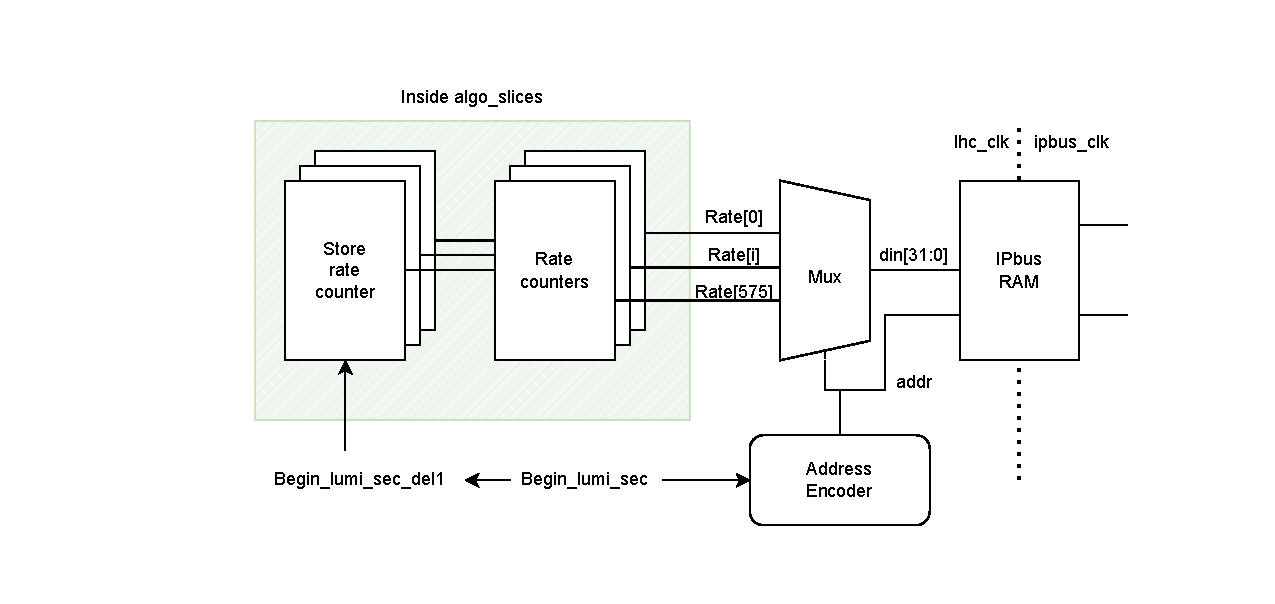
\includegraphics[width=0.8\textwidth]{sections/06/Images/Rate_regs.pdf}
    \caption{Optimization done in the rate counters reading}
    \label{fig:Rate_cnt}
\end{figure}

Four rate counter are instantiated for each algorithm, one before the pre-scale, one after the pre-scale, one after the preview pre-scale and one post dead-time. The post dead-time counter is a slight variation of the other three, it increments the register only if the algorithm and the delayed L1A signal are both asserted,  which means that only the algorithm assertions that can save the event are taking into account.

\subsection{Trigger masks and final-OR}
\label{sec:Finor_trigger}

Unlike $\mu$GT the Phase-2 GT will have multiple trigger bits which are selected to tackle different Physics, an example of 8 trigger bits is given in the table \ref{tab:trigger_types} \cite{L1T-2up}.  


\begin{table}[ht] \
  \begin{minipage}[b]{0.5\linewidth}
    \centering
    \begin{tabular}{|c|c|}
    \hline
    Index & Trigger type      \\
    \hline
    0 & Stadard Physics     \\
    1 & Zero Bias           \\
    2 & Minimum Bias            \\
    3 & High Priority       \\
    4 & Long-lived particle (LLP)    \\
    5 & First event of a 2-event LLP   \\
    6 & Second event of a 2-event LLP  \\
    7 & Periodic validation event      \\
    \hline
    \end{tabular}
    \caption{Example of 8 different trigger bits}
    \label{tab:trigger_types}
    \vspace{4ex}
  \end{minipage}%%
  \begin{minipage}[b]{0.5\linewidth}
    \centering
    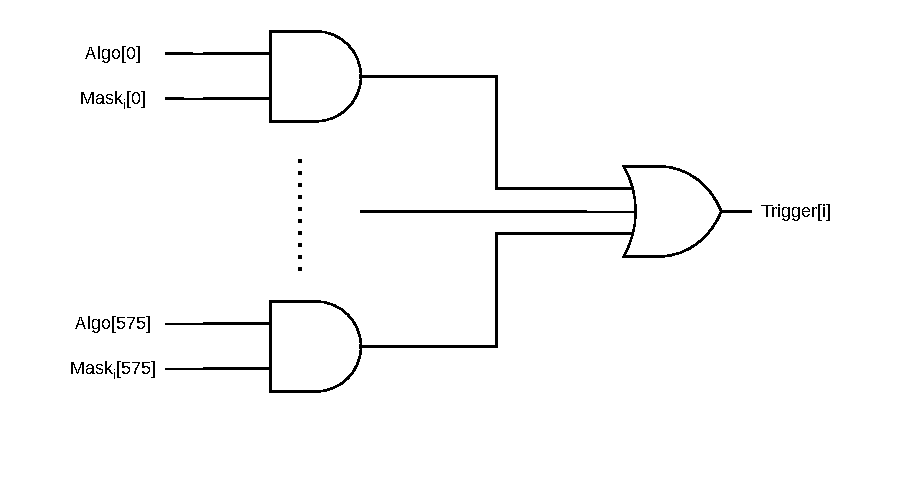
\includegraphics[width=0.95\textwidth]{sections/06/Images/TriggerMasks.pdf}
    \captionof{figure}{Schematic view of the extraction of the i-esim local trigger bit.}
    \label{fig:TriggMasks}
    \vspace{4ex}
  \end{minipage} 
\end{table}

To extract such trigger bits, first a mask is applied to the whole algorithm vector selecting only a fraction of the 576 bits\footnote{This process is done in each monitoring SLR}, then local OR\footnote{Local in the sens that is computed in each SLR} is computed to each masks results, such outputs are the local trigger bits. The masks are loaded via an IPbus dual port RAM with the exact same structure of the pre-scale factors. A diagram of such process is shown in Fig. \ref{fig:TriggMasks}

\begin{figure}[!h]
    
\end{figure}

\clearpage
\section{Final-OR board standalone test}
\label{sec:Finor_standalone}

The design described in the previous sections has been tested in a different way with respect to the other boards, in fact the output pattern is not checked against one produced in simulation or emulation. The aim of this test is to test every single algorithm index whereas the final output does not give any information on how a single algorithm slice behaves.  

\begin{figure}[!h]
    \centering
    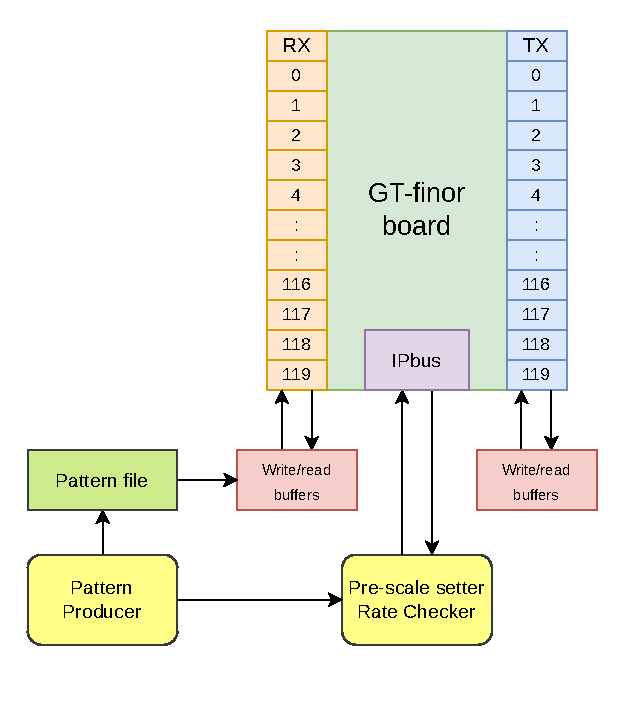
\includegraphics[width=0.6\textwidth]{sections/06/Images/Finor_test.pdf}
    \caption{GT Final-OR standalone board test. A pattern is produced alongside a pre-scale column, then the pattern is loaded and the result are checked against the expected ones.}
    \label{fig:Finor_board_test}
\end{figure}

A pattern file contains exactly 1024 frames due to the buffer dimension, each frame is the ensemble of the data sent through the datapath input buffers in one link clock (360MHz), which means that a bunch crossing contains nine frames and a total of 576 bits per link. A pattern file contains 113 bunch crossing\footnote{Nearest integer of the ratio 1024/9}. During the hardware test this pattern file is reproduced at the beginning of each orbit. The maximum number of algorithm assertion that is possible to send with this configuration in a luminosity section is:

\begin{equation}
    algo_{max}^{test} = 113\cdot2^{19} = 59244544\\
    \label{eq:max_ass}
\end{equation}


The hardware setup is sketched in Fig. \ref{fig:Finor_board_test}, the workflow is the following:
\begin{itemize}
    \item A number of algorithm indexes is declared with a random number of assertions -from 0 to 113- for each index extracted;
    \item A pattern file is produced from the selected indexes, the algorithm are distributed to the various suitable input links;
    \item A set of pre-scale values\footnote{In the CMS literature this set is usually called pre-scale column} is loaded;
    \item The pattern file is loaded and the board is set to run continuously;
    \item At the beginning of each luminosity section the rate counters are read;
    \item Finally the rate counters before and after the pre-scales are divided to obtain the pre-scale factors and compared with the pre-scale column. If the match is reached the test is completed successfully. 
\end{itemize}

%\vfill
\subsection{Result}
In table \ref{tab:Finor_res} are shown the results of the final OR standalone test, multiple pattern files were tested with different number of algorithm indexes.
The \textit{random pre-scaler} test set up a random value for each pre-scaler, the test is left run for 20 luminosity section, corresponding to $\sim$930 seconds. 
This test is considered pass only if perfect match is obtained.


\begin{table}[h]
    \centering
    \begin{tabular}{|c|c|c|c|}
    \hline
    N Algorithms injected & Test type  & Duration [s]&  Outcome \\
    \hline
    10          & Random Pre-scaler    & 932 & Pass             \\
    50          & Random Pre-scaler    & 932 & Pass             \\
    100         & Random Pre-scaler    & 932 & Pass             \\
    500         & Random Pre-scaler    & 932 & Pass             \\
    1000        & Random Pre-scaler    & 932 & Pass             \\
    1152        & Random Pre-scaler    & 932 & Pass             \\
    \hline
    \end{tabular}
    \caption{Final or pre-scaer test results.}
    \label{tab:Finor_res}
\end{table}

\vfill
        
\section{Multi-board test}
\label{sec:Finor_multiboard}
The last hardware test would be the whole Global Trigger system, in other words the two different boards are connected together to simulate the real layout that will be deployed in the Phase-II Global Trigger.
\begin{itemize}
    \item \textbf{Algo-board}: this board will take as inputs the output of the pattern files produced by the upstream system emulator, the algorithm and the neural network conditions are computed and the relative algo-bits are sent as output to the finor-board;
    \item \textbf{Finor-board}: last element of the chain, here the algorithms are pre-scaled and the rates are extracted, then the rates will be checked afterward against the expected ones; in this step it is also possible to test the trigger masks and the relative final decisions rates.
\end{itemize}

\begin{figure}[h]
    \centering
    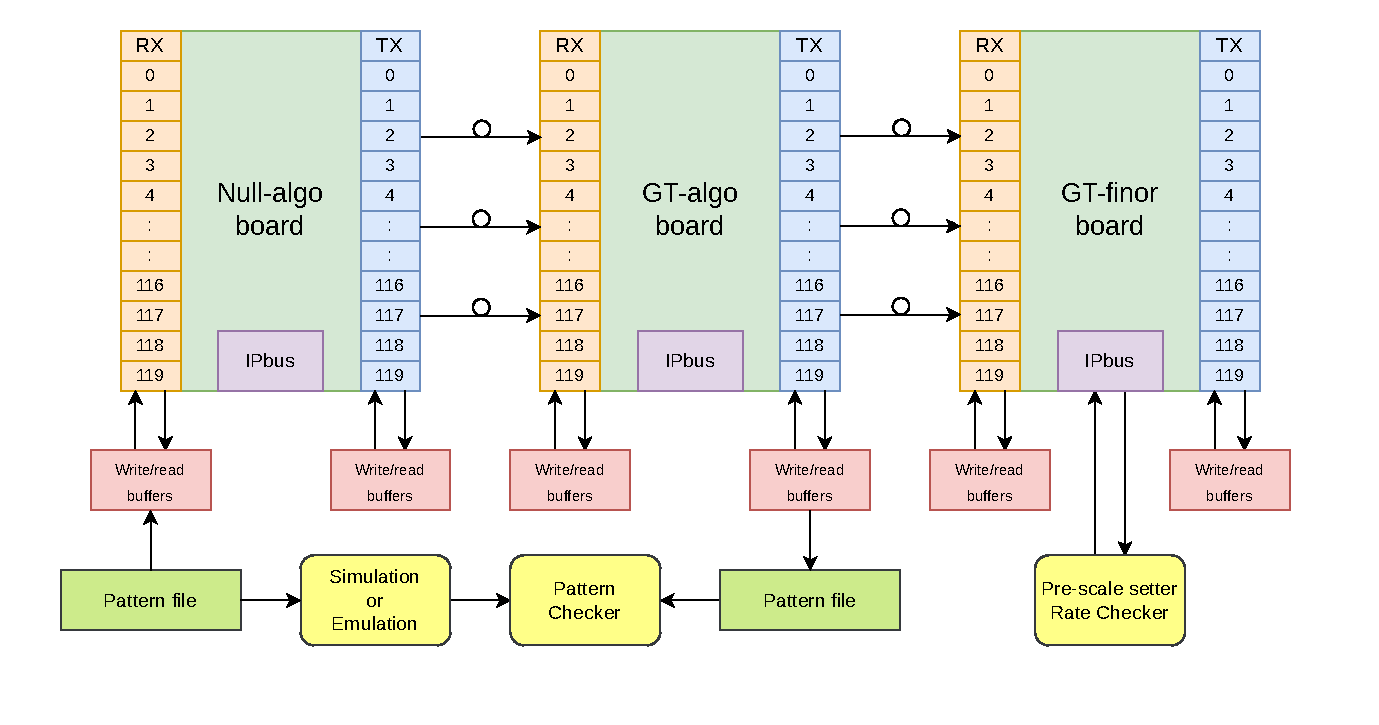
\includegraphics[width=0.9\textwidth]{sections/06/Images/Board_test.pdf}
    \caption{Two-board test.}
    \label{fig:Two_board_test}
\end{figure}

In Fig. \ref{fig:Two_board_test} the two boards connection is shown. A pattern is produced by the upstream emulator, then it is loaded in the input buffers of the algo-board. The algo-board computes the algorithms and the relative algo-bits are sent to the finor-board, here the pre-scales are applied and the rate are extracted. Outputs are checked both in the algo-board and in the finor-board.

This test is meant to check the outputs in two points, one right after the algo-board and one on the finor-board IPbus register values.  
The pattern file contains the data coming from the upstream systems, a pattern producer is employed to obtain such file with the \acrfull{cl2} and \acrfull{gmt} time multiplexed data.  


\subsection{Result}

The input pattern file contains the data coming from the CL2 and GMT subsystems, in particular it contains a small data sample taken from the test data set described in section \ref{sec:NN-dataset}. Due to hardware limitations only 72 data samples were injected\footnote{EMP framework does not yet support complex pattern injection, a solution could be an auxiliary board with large memory buffers as a pattern producer}. A number of algorithms are computed to produce a small trigger menu, the list is given in the table \ref{tab:test_algos}. Only the best performing neural networks per leptonic channel were tested. The algorithm menu is replicated exactly in each of the three SLRs, while only the SLR$_2$ output was considered for the test due to limited connection between the test boards.  

The counts are extracted from the finor board register bank an then compared to the results obtained in software. In particular QKeras, Numpy and CMSSW were used for neural networks, cut based algorithms and GT emulation respectively.

\begin{table}[h]
    \centering
    \begin{tabular}{|c|c|c|c|c|c|}
    \hline
    Algorithm & Index & Notes & Assertion/orbit & Counts$_{Theo}$ & Counts$_{Test}$ \\
    \hline
    Single Muon      &0& $p_T \geq 20GeV$            & 11 & 5767168  & 5767168   \\
    Single Electron  &1& $p_T \geq 30GeV$            & 6  & 3145728 &  3145728 \\
    Single PuppiJet  &2& $p_T \geq 163GeV$              & 11 & 5767168 & 5767168  \\
    Double Muon      &3& $p_T^{0-1} \geq 14,6GeV$    & 8  & 4194304  & 4194304   \\
    Double Electron  &4& $p_T^{0-1} \geq 21,10GeV$   & 1  & 524288  & 524288  \\
    Double PuppiJet  &5& $p_T^{0-1} \geq 75,75GeV$ & 17 & 8912896 & 8912896  \\
    \hline
    %NN 3 layers      &6& $e$ channel  & 10485760 & 10485760 \\
    %NN 2 layers      &7& $e$ channel  & 9437184  & 9437184  \\
    NN 1 layer       &6& $e$ channel  & 23 & 12058624 & 12058624 \\
    %NN 16 nodes      &9& $e$ channel  & 10485760 & 10485760 \\
    %BNN              &10& $e$ channel & 9437184 & 9437184 \\
    %TNN              &11& $e$ channel & 9961472 & 9961472 \\
    \hline
    %NN 3 layers      &12& $\mu$ channel & 9961472  & 9961472 \\
    %NN 2 layers      &13& $\mu$ channel & 9961472  & 9961472 \\
    NN 1 layer       &7& $\mu$ channel & 23 & 12058624  & 12058624 \\
    %NN 16 nodes      &15& $\mu$ channel & 9961472  & 9961472 \\
    %BNN              &16& $\mu$ channel & 10485760 & 10485760 \\
    %TNN              &17& $\mu$ channel & 10485760 & 10485760 \\
    \hline
    \end{tabular}
    \caption{Example of a simplified menu containing the neural network based conditions}
    \label{tab:test_algos}
\end{table}

The counts extracted have perfect match with software counterparts, the test is considered accomplished.
    

\end{document}